\ylDisplay{Kaks valgusallikat} % Ülesande nimi
{EFO žürii} % Autor
{piirkonnavoor} % Voor
{2018} % Aasta
{P 9} % Ülesande nr.
{3} % Raskustase
{
% Teema: Valgusõpetus
\ifStatement
Kaks punktikujulist valgusallikat asuvad kumerläätse optilisel peateljel erinevates punktides. Nendest valgusallikatest läätse abil tekitatud kujutised kattuvad. On teada, et üks valgusallikas asub läätse keskpunktist $a = 18$ cm kaugusel. Kui kaugel sellest valgusallikast asub teine valgusallikas? Läätse fookuskaugus $f = 9$ cm.
\fi
\ifHint
Kui optilisel peateljel paiknev valgusallikas asub läätsest $18$ cm kaugusel, mis on võrdne kahekordse fookuskaugusega, siis selle valgusallika kujutis asub teisel pool läätse läätsest samuti kahe fookuskaugusel. Et kahe valgusallika kujutised kattuksid, peab teine kujutis olema näilik. Ülesanne lahendub lbäi sarnaste kolmnurkade seoste.
\fi
\ifSolution
Kui optilisel peateljel paiknev valgusallikas asub läätsest $18$ cm kaugusel, mis on võrdne kahekordse fookuskaugusega, siis selle valgusallika kujutis asub teisel pool läätse läätsest samuti kahe fookuskaugusel ehk $18$ cm kaugusel. Et kahe valgusallika kujutised kattuksid, peab teine kujutis olema näilik. Konstrueerime valgusallika asukoha, kui kujutise asukoht on teada.
Sarnastest kolmnnurkadest $\triangle KAO$ ja $\triangle KBF$ saame, et 
\begin{center}
$\frac{AO}{BF} = \frac{KO}{KF} = \frac{2f}{3f} = \frac{2}{3}$.
\end{center}
Teisest sarnaste kolmnurkade paarist $\triangle SAO$ ja $\triangle OBF$ saame, et 
\begin{center}
$\frac{AO}{BF} = \frac{OS}{FO} = \frac{b}{f}$,
\end{center}
kus $b$ - teise valgusallika kaugus läätsest. Ühendades kaks seost saame:
\begin{center}
$\frac{KO}{KF}$ $\Rightarrow$ $\frac{OS}{FO}$ $\Rightarrow$ $b = \frac{2f}{3} = 6$ cm.
\end{center}
Teine valgusallikas peab asetsema läätsest $6$ $cm$ kaugusel ning kahe valgusallika kaugus teineteisest on $6 cm + 18 cm = 24$ cm.
\begin{center}
	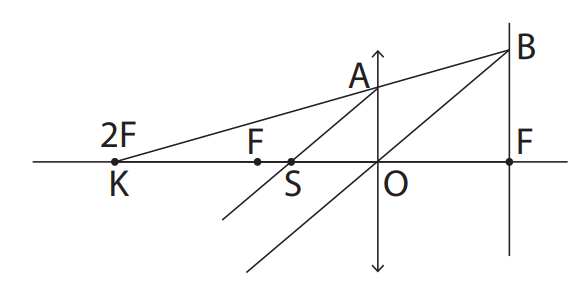
\includegraphics[width=0.5\linewidth]{2018-v2p-09-lah.PNG}
\end{center}
\fi
}
